\let\negmedspace\undefined
\let\negthickspace\undefined
\documentclass[journal,12pt,onecolumn]{IEEEtran}
%\documentclass[conference]{IEEEtran}
%\IEEEoverridecommandlockouts
% The preceding line is only needed to identify funding in the first footnote. If that is unneeded, please comment it out.
\usepackage{cite}
\usepackage{amsmath,amssymb,amsfonts,amsthm}
\usepackage{algorithmic}
\usepackage{graphicx}
\usepackage{textcomp}
\usepackage{xcolor}
\usepackage{txfonts}
\usepackage{listings}
\usepackage{enumitem}
\usepackage{mathtools}
\usepackage{gensymb}
\usepackage[breaklinks=true]{hyperref}
\usepackage{tkz-euclide} % loads  TikZ and tkz-base
\usepackage{listings}
\usepackage{breqn}
%
%\usepackage{setspace}
%\usepackage{gensymb}
%\doublespacing
%\singlespacing

%\usepackage{graphicx}
%\usepackage{amssymb}
%\usepackage{relsize}
%\usepackage[cmex10]{amsmath}
%\usepackage{amsthm}
%\interdisplaylinepenalty=2500
%\savesymbol{iint}
%\usepackage{txfonts}
%\restoresymbol{TXF}{iint}
%\usepackage{wasysym}
%\usepackage{amsthm}
%\usepackage{iithtlc}
%\usepackage{mathrsfs}
%\usepackage{txfonts}
%\usepackage{stfloats}
%\usepackage{bm}
%\usepackage{cite}
%\usepackage{cases}
%\usepackage{subfig}
%\usepackage{xtab}
\usepackage{longtable}
\usepackage{multirow}
%\usepackage{algorithm}
%\usepackage{algpseudocode}
%\usepackage{enumitem}
%\usepackage{mathtools}
\usepackage{tikz}
%\usepackage{circuitikz}
%\usepackage{verbatim}
%\usepackage{tfrupee}
%\usepackage{stmaryrd}
%\usetkzobj{all}
%    \usepackage{color}                                            %%
%    \usepackage{array}                                            %%
%    \usepackage{longtable}                                        %%
%    \usepackage{calc}                                             %%
%    \usepackage{multirow}                                         %%
    \usepackage{hhline}                                           %%
    \usepackage{ifthen}                                           %%
  %optionally (for landscape tables embedded in another document): %%
%    \usepackage{lscape}     
\usepackage{multicol}
%\usepackage{chngcntr}
\usepackage{enumerate}

%\usepackage{wasysym}
%\newcounter{MYtempeqncnt}
\DeclareMathOperator*{\Res}{Res}
%\renewcommand{\baselinestretch}{2}
\renewcommand\thesection{\arabic{section}}
\renewcommand\thesubsection{\thesection.\arabic{subsection}}
\renewcommand\thesubsubsection{\thesubsection.\arabic{subsubsection}}

\renewcommand\thesectiondis{\arabic{section}}
\renewcommand\thesubsectiondis{\thesectiondis.\arabic{subsection}}
\renewcommand\thesubsubsectiondis{\thesubsectiondis.\arabic{subsubsection}}

% correct bad hyphenation here
\hyphenation{op-tical net-works semi-conduc-tor}
\def\inputGnumericTable{}                                 %%

\lstset{
%language=C,
frame=single, 
breaklines=true,
columns=fullflexible
}
%\lstset{
%language=tex,
%frame=single, 
%breaklines=true
%}

\begin{document}
%


\newtheorem{theorem}{Theorem}[section]
\newtheorem{problem}{Problem}
\newtheorem{proposition}{Proposition}[section]
\newtheorem{lemma}{Lemma}[section]
\newtheorem{corollary}[theorem]{Corollary}
\newtheorem{example}{Example}[section]
\newtheorem{definition}[problem]{Definition}
%\newtheorem{thm}{Theorem}[section] 
%\newtheorem{defn}[thm]{Definition}
%\newtheorem{algorithm}{Algorithm}[section]
%\newtheorem{cor}{Corollary}
\newcommand{\BEQA}{\begin{eqnarray}}
\newcommand{\EEQA}{\end{eqnarray}}
\newcommand{\define}{\stackrel{\triangle}{=}}
\bibliographystyle{IEEEtran}
%\bibliographystyle{ieeetr}
\providecommand{\mbf}{\mathbf}
\providecommand{\pr}[1]{\ensuremath{\Pr\left(#1\right)}}
\providecommand{\qfunc}[1]{\ensuremath{Q\left(#1\right)}}
\providecommand{\sbrak}[1]{\ensuremath{{}\left[#1\right]}}
\providecommand{\lsbrak}[1]{\ensuremath{{}\left[#1\right.}}
\providecommand{\rsbrak}[1]{\ensuremath{{}\left.#1\right]}}
\providecommand{\brak}[1]{\ensuremath{\left(#1\right)}}
\providecommand{\lbrak}[1]{\ensuremath{\left(#1\right.}}
\providecommand{\rbrak}[1]{\ensuremath{\left.#1\right)}}
\providecommand{\cbrak}[1]{\ensuremath{\left\{#1\right\}}}
\providecommand{\lcbrak}[1]{\ensuremath{\left\{#1\right.}}
\providecommand{\rcbrak}[1]{\ensuremath{\left.#1\right\}}}
\theoremstyle{remark}
\newtheorem{rem}{Remark}
\newcommand{\sgn}{\mathop{\mathrm{sgn}}}
\providecommand{\abs}[1]{\left\vert#1\right\vert}
\providecommand{\res}[1]{\Res\displaylimits_{#1}} 
\providecommand{\norm}[1]{\left\lVert#1\right\rVert}
%\providecommand{\norm}[1]{\lVert#1\rVert}
\providecommand{\mtx}[1]{\mathbf{#1}}
\providecommand{\mean}[1]{E\left[ #1 \right]}
\providecommand{\fourier}{\overset{\mathcal{F}}{ \rightleftharpoons}}
%\providecommand{\hilbert}{\overset{\mathcal{H}}{ \rightleftharpoons}}
\providecommand{\system}{\overset{\mathcal{H}}{ \longleftrightarrow}}
	%\newcommand{\solution}[2]{\textbf{Solution:}{#1}}
\newcommand{\solution}{\noindent \textbf{Solution: }}
\newcommand{\cosec}{\,\text{cosec}\,}
\providecommand{\dec}[2]{\ensuremath{\overset{#1}{\underset{#2}{\gtrless}}}}
\newcommand{\myvec}[1]{\ensuremath{\begin{pmatrix}#1\end{pmatrix}}}
\newcommand{\mydet}[1]{\ensuremath{\begin{vmatrix}#1\end{vmatrix}}}
%\numberwithin{equation}{section}
%\numberwithin{equation}{subsection}
%\numberwithin{problem}{section}
%\numberwithin{definition}{section}
%\makeatletter
%\@addtoreset{figure}{problem}
%\makeatother
%\let\StandardTheFigure\thefigure
\let\vec\mathbf
%\renewcommand{\thefigure}{\theproblem.\arabic{figure}}
%\renewcommand{\thefigure}{\theproblem}
%\setlist[enumerate,1]{before=\renewcommand\theequation{\theenumi.\arabic{equation}}
%\counterwithin{equation}{enumi}
%\renewcommand{\theequation}{\arabic{subsection}.\arabic{equation}}
%\def\putbox#1#2#3{\makebox[0in][l]{\makebox[#1][l]{}\raisebox{\baselineskip}[0in][0in]{\raisebox{#2}[0in][0in]{#3}}}}
%     \def\rightbox#1{\makebox[0in][r]{#1}}
%     \def\centbox#1{\makebox[0in]{#1}}
%     \def\topbox#1{\raisebox{-\baselineskip}[0in][0in]{#1}}
%     \def\midbox#1{\raisebox{-0.5\baselineskip}[0in][0in]{#1}}
\vspace{3cm}
\title{
%	\logo{
\textbf {Assignment 2} \\ \large \textbf{AI1110} : Probability and Random Variables \\ Indian Institute of Technology Hyderabad
%	}
}
\author{Manpurwar Ganesh*% <-this % stops a space
	\thanks{*The studnent is with the Department
		of AI , Indian Institute of Technology, Hyderabad
		502285 India e-mail: ai22btech11017@iith.ac.in.}
	
}	
%\title{
%	\logo{Matrix Analysis through Octave}{\begin{center}\includegraphics[scale=.24]{tlc}\end{center}}{}{HAMDSP}
%}
% paper title
% can use linebreaks \\ within to get better formatting as desired
%\title{Matrix Analysis through Octave}
%
%
% author names and IEEE memberships
% note positions of commas and nonbreaking spaces ( ~ ) LaTeX will not break
% a structure at a ~ so this keeps an author's name from being broken across
% two lines.
% use \thanks{} to gain access to the first footnote area
% a separate \thanks must be used for each paragraph as LaTeX2e's \thanks
% was not built to handle multiple paragraphs
%
%\author{<-this % stops a space
%\thanks{}}
%}
% note the % following the last \IEEEmembership and also \thanks - 
% these prevent an unwanted space from occurring between the last author name
% and the end of the author line. i.e., if you had this:
% 
% \author{....lastname \thanks{...} \thanks{...} }
%                     ^------------^------------^----Do not want these spaces!
%
% a space would be appended to the last name and could cause every name on that
% line to be shifted left slightly. This is one of those "LaTeX things". For
% instance, "\textbf{A} \textbf{B}" will typeset as "A B" not "AB". To get
% "AB" then you have to do: "\textbf{A}\textbf{B}"
% \thanks is no different in this regard, so shield the last } of each \thanks
% that ends a line with a % and do not let a space in before the next \thanks.
% Spaces after \IEEEmembership other than the last one are OK (and needed) as
% you are supposed to have spaces between the names. For what it is worth,
% this is a minor point as most people would not even notice if the said evil
% space somehow managed to creep in.
% The paper headers
%\markboth{Journal of \LaTeX\ Class Files,~Vol.~6, No.~1, January~2007}%
%{Shell \MakeLowercase{\textit{et al.}}: Bare Demo of IEEEtran.cls for Journals}
% The only time the second header will appear is for the odd numbered pages
% after the title page when using the twoside option.
% 
% * Note that you probably will NOT want to include the author's *
% * name in the headers of peer review papers.                   *
% You can use \ifCLASSOPTIONpeerreview for conditional compilation here if
% you desire.
% If you want to put a publisher's ID mark on the page you can do it like
% this:
%\IEEEpubid{0000--0000/00\$00.00~\copyright~2007 IEEE}
% Remember, if you use this you must call \IEEEpubidadjcol in the second
% column for its text to clear the IEEEpubid mark.
% make the title area
\maketitle
%\tableofcontents
\bigskip
\renewcommand{\thefigure}{\theenumi}
\renewcommand{\thetable}{\theenumi}
%\renewcommand{\theequation}{\theenumi}
%\begin{abstract}
%%\boldmath
%In this letter, an algorithm for evaluating the exact analytical bit error rate  (BER)  for the piecewise linear (PL) combiner for  multiple relays is presented. Previous results were available only for upto three relays. The algorithm is unique in the sense that  the actual mathematical expressions, that are prohibitively large, need not be explicitly obtained. The diversity gain due to multiple relays is shown through plots of the analytical BER, well supported by simulations. 
%
%\end{abstract}
% IEEEtran.cls defaults to using nonbold math in the Abstract.
% This preserves the distinction between vectors and scalars. However,
% if the journal you are submitting to favors bold math in the abstract,
% then you can use LaTeX's standard command \boldmath at the very start
% of the abstract to achieve this. Many IEEE journals frown on math
% in the abstract anyway.
% Note that keywords are not normally used for peerreview papers.
%\begin{IEEEkeywords}
%Cooperative diversity, decode and forward, piecewise linear
%\end{IEEEkeywords}
% For peer review papers, you can put extra information on the cover
% page as needed:
% \ifCLASSOPTIONpeerreview
% \begin{center} \bfseries EDICS Category: 3-BBND \end{center}
% \fi
%
% For peerreview papers, this IEEEtran command inserts a page break and
% creates the second title. It will be ignored for other modes.
%\IEEEpeerreviewmaketitle
%%%%%%%%%%%%%%%%%%%%%  This is my Assignment %%%%%%%%%%%%%%%%%%%%%

\title{ Random Number Generator Using Electronic Components}
\author{MANPURWAR GANESH \\AI22BTECH11017}
\date{\today}


\maketitle

\section{Introduction}
The objective of this lab experiment was to design and build a random number generator that generates a single-digit random number using a breadboard and various electronic components. The key components utilized in this project included a breadboard, seven-segment display, 7474 flip-flop, 7447 decoder, 7684 clock, 555 IC, resistors (1kohm, 1mohm), capacitors (100nf, 10nf), and jump wires. This report presents a concise description of the circuit, along with an output image and a block diagram, to illustrate the construction and functionality of the single-digit random number generator.

\section{List of Components}
The following components were used in the construction of the single-digit random number generator:\\
\begin{tabular}{|l|l|l|}
\hline
component&value&quantity\\
\hline
Breadboard & & 1\\
\hline
Seven-segment display& common anode& 1\\
\hline
 flip-flop& 7474 &2\\
 \hline
 decoder& 7447 &1\\
 \hline
X-OR GATE& 7684 &1 \\
\hline
555 IC& &1\\
\hline
 Resistor& 1kohm &1\\
 \hline
 Resistor& 1mohm &1\\
 \hline
 Capacitor& 100nf &1\\
 \hline
 Capacitor&10nf &1\\
 \hline
 Jump wires& &20\\
 \hline
\end{tabular}
\section{Circuit Description}
The single-digit random number generator circuit was designed to generate a random number ranging from 0 to 9 using a combination of flip-flops, decoders, clocks, and other electronic components. The circuit operation can be summarized as follows:

\begin{itemize}
    \item The circuit operates with a 5V power supply obtained from a micro USB connection. This voltage, referred to as Vcc, serves as the power source for the entire circuit. The OUTERMOST buses on both sides of the circuit carries the Clock signal generated by a 555 precision timer. The upper inner bus is connected to the vcc. The lower inner bus is connected to the GRD.

    \item The 555 IC was configured as an astable multivibrator, generating a continuous stream of clock pulses. The resistor R1 (1kohm) and capacitor C1 (10nf) were carefully selected to determine the frequency of the clock pulses. These components were chosen to provide a suitable timing range for the random number generation process while ensuring that the output is limited to a single digit.
    
    \item The clock pulses were then fed into the 7684 clock module, which acted as a clock divider. This module divided the input clock frequency to produce slower clock cycles, allowing for precise control and synchronization within the circuit.
    
    \item The slower clock cycles were directed to the clock input of the 7474 flip-flop. This flip-flop, together with its associated capacitor C2 (100nf), provided buffering and stabilization for reliable operation. Capacitor C2 filtered any potential noise from the clock signal, ensuring stable voltage levels within the flip-flop.
    
    \item The outputs of the flip-flop were connected to the inputs of the 7447 decoder. This decoder, in combination with the resistor R2 (1kohm), decoded the binary outputs from the flip-flop into the appropriate signals for driving the seven-segment display. The resistor R2 was used to limit the current flowing through the decoder's input, preventing any damage to the components.
    
    \item Finally, the seven-segment display was connected to the decoder's outputs. It visually represented the generated random number in decimal format, displaying a single digit ranging from 0 to 9. The decoder and display were configured to ensure that only one digit would be shown at a time.
\end{itemize}

By employing this circuit configuration, the random number generator was able to reliably generate single-digit random numbers based on the timing of the clock pulses and the state of the flip-flop outputs.

\section{Output Image}
\begin{figure}[ht]
  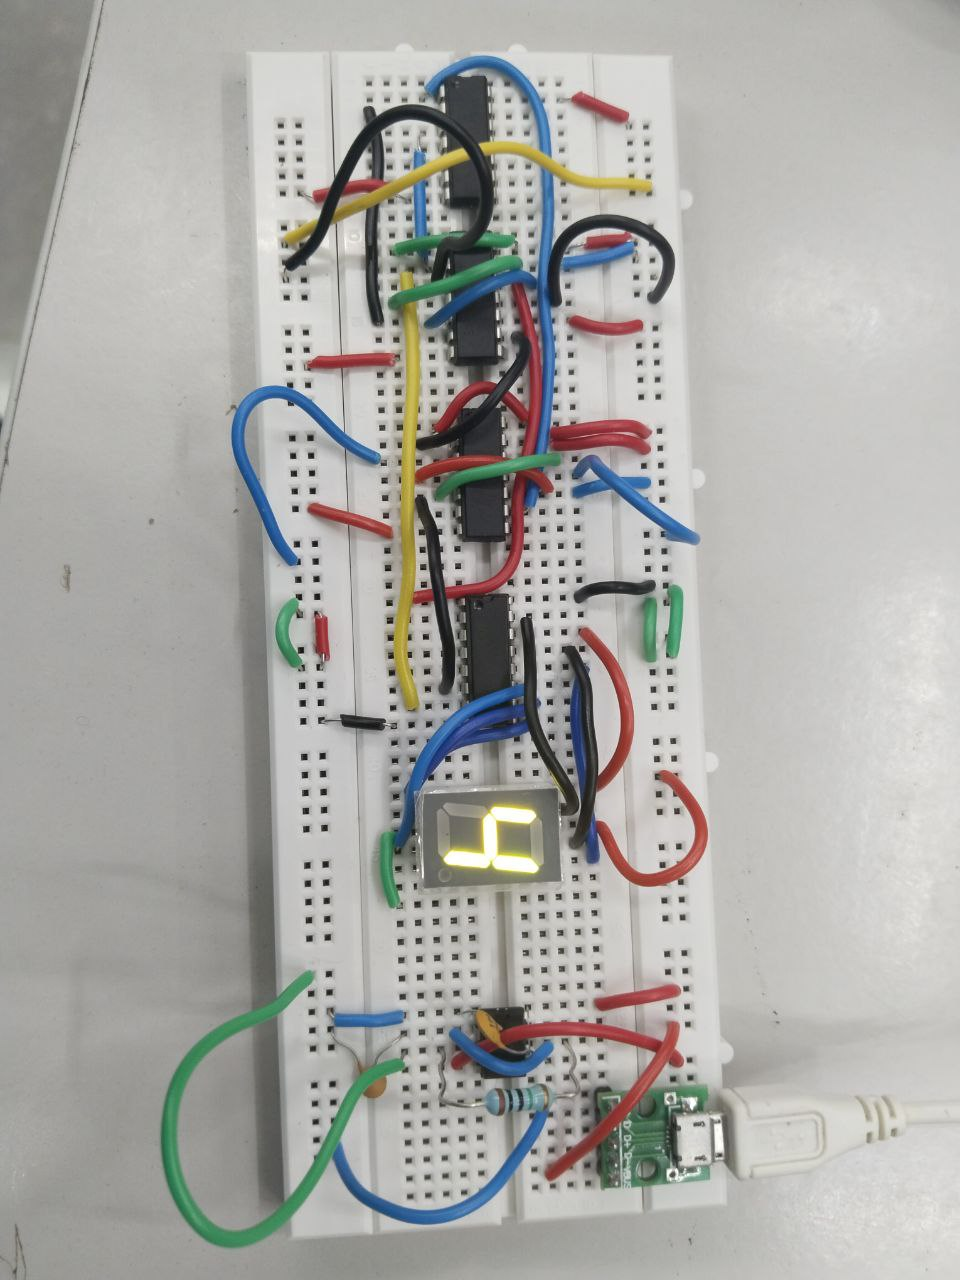
\includegraphics[width=5cm]{/home/ganesh/Hardware/images/4.jpg}
  \caption{ output 1}
  \label{SSD}
 \end{figure}
\begin{figure}[ht]
  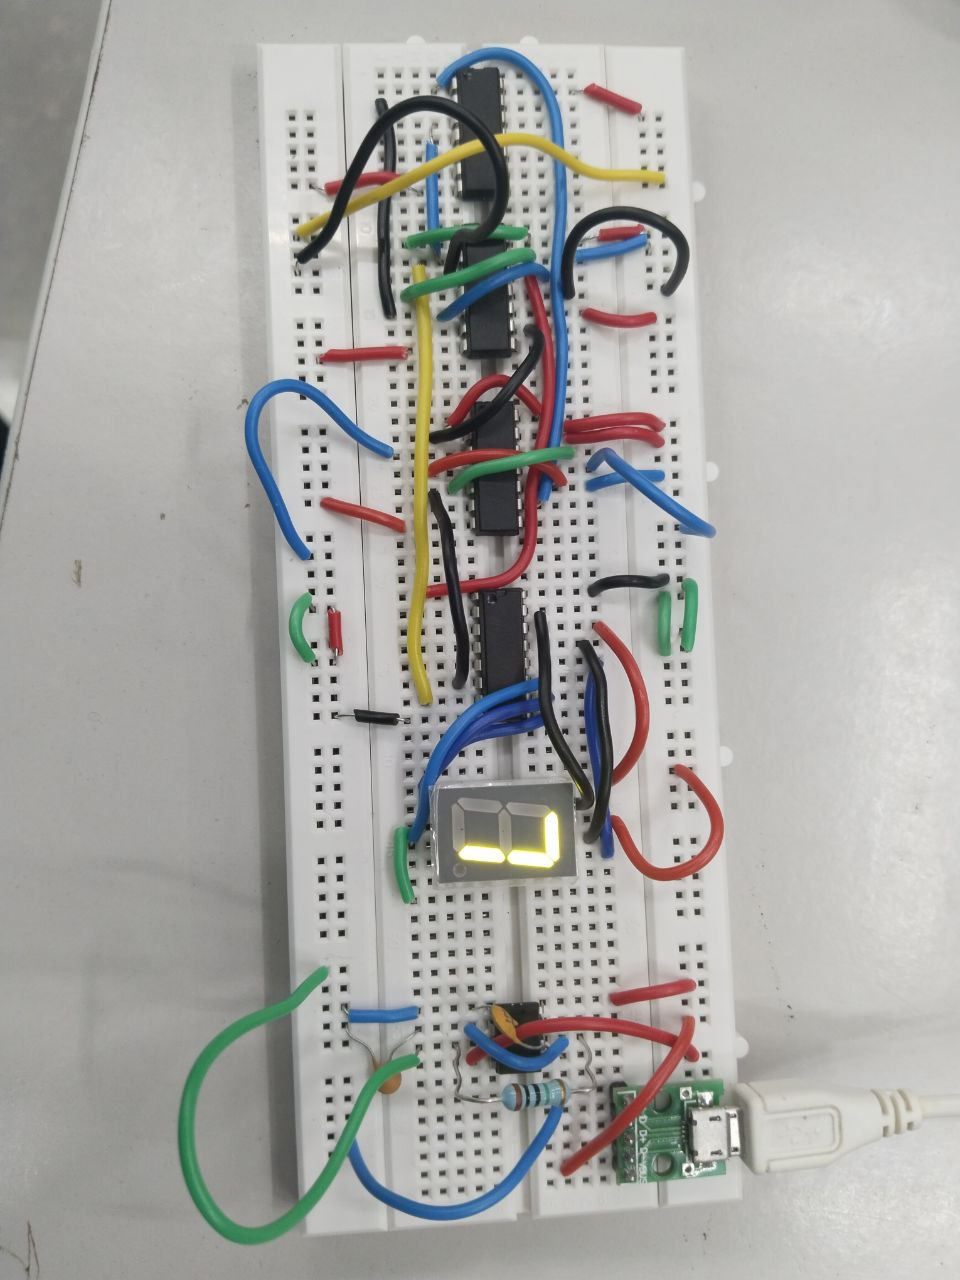
\includegraphics[width=5cm]{/home/ganesh/Hardware/images/7.jpg}
  \caption{output 2}
  \label{SSD}
 \end{figure}
 \begin{figure}[ht]
  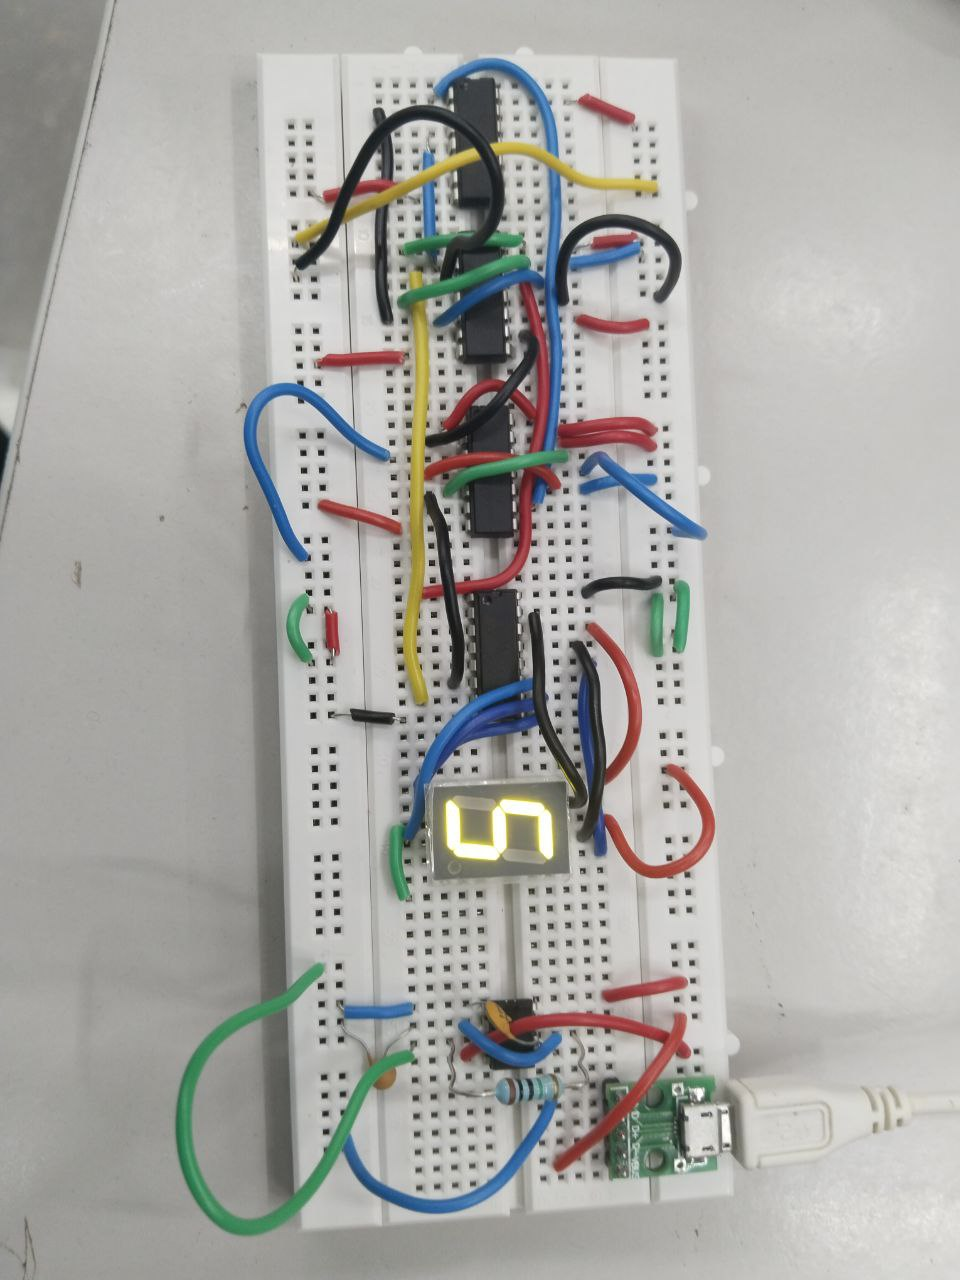
\includegraphics[width=5cm]{/home/ganesh/Hardware/images/5.jpg}
  \caption{output 3}
  \label{SSD}
 \end{figure}

\begin{figure}[ht]
  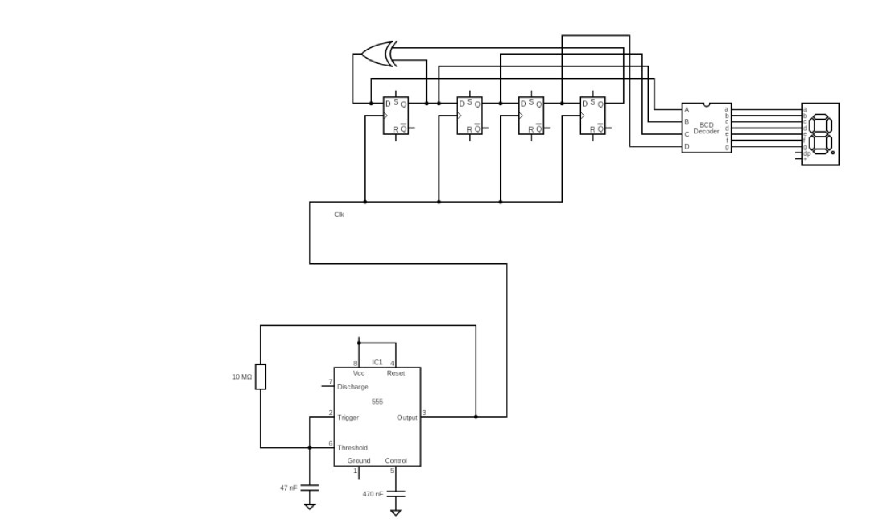
\includegraphics[width=20cm]{/home/ganesh/block diagram.png}
  \caption{BLOCK DIAGRAM}
  \label{SSD}
 \end{figure}
\vspace{10cm}
\section{Conclusion}
This lab experiment successfully demonstrated the construction of a single-digit random number generator using a breadboard and a combination of electronic components. The designed circuit, consisting of the 555 IC, 7684 clock, 7474 flip-flop, 7447 decoder, and seven-segment display, effectively generated random numbers in the range of 0 to 9. 
\end{document}
